\chapter{SLAM Pipeline}

If we consider mobile robotics to be comprised of: "Where am I", "Where am I going", and "How do I get there", SLAM answers the first (Leonard and Durrant Whyte). So, what is SLAM? A robot observes the environment relative to its unknown pose, this helps localise the position. On the other hand, if we know our location, we can create a map of the environment based on the sensor inputs we have. Hence, the simultaneous localization and mapping. 

I really really liked \href{http://www.informatik.uni-bremen.de/agebv2/downloads/published/freseki10.pdf}{this paper that explains SLAM from a user perspective}. It abstracts the math away for a while, to focus on the bigger picture.

"The  need  to  use  a  map  of  the  environment  is  twofold. First,  the  map is  often  required  to  support  other  tasks;  for instance,  a  map  can  inform  path  planning  or  provide  an intuitive visualization for a human operator. Second, the map allows limiting the error committed in estimating the state of the  robot.  In  the  absence  of  a  map,  dead-reckoning  would quickly drift over time; on the other hand, using a map, e.g.,a  set  of  distinguishable  landmarks,  the  robot  can  “reset”  its localization  error  by  re-visiting  known  areas  (so-called loop closure). Therefore, SLAM finds applications in all scenarios in which a prior map is not available and needs to be built." from \href{https://arxiv.org/pdf/1606.05830.pdf#page=1&zoom=auto,-18,801}{ a review paper}

\section{The Big Picture \& State of the Art}

First, based on data received by the sensors we will extract features. These features are then passed to a data association block which tracks features (short term) and loop closure (long term with bag of visual words). Feature tracking is essentially feature matching (optical flow) between two close frames. Visual odometry is then done after feature tracking to calculate the transformations between robot poses. If we have sensors like wheel odometry, we can also do EKF fusion - gives us a better estimate of wheel odometry. There are some packages which also perform local bundle adjustment. The output of the frontend is keyframe poses and loop closure pairs which feeds into the backend.

The backend will then optimize the results given by frontend and obtain optical relative transformation. The global map is then assembled based on optimized poses and local point clouds.

As per the review paper mentioned earlier, the frontend is where SLAM meets other research fields - computer vision and signal processing, the backend is more mathematical and involves optimizations, and probabilistic estimation.

One key thing to note when looking at the loop closure section is that it makes SLAM unique. Otherwise, this is just an odometry problem. 

\section{Iterative Closest Points}

Let's say that we have a vehicle which is moving and constantly taking pictures of the world around it. It has some features or point clouds with respect to the frames at two different instances. Now, if we want to figure out the transformation between these two frames, how do we go about it? ICP is the task of finding parameters of the transformation that best aligns corresponding data points. Or estimating our state using point set registration. We usually solve this as an optimization problem, where we have two sets of points, and a hypothetical transformation between them. So with a series of equations, we can solve for a solution.

\begin{figure}
    \centering
    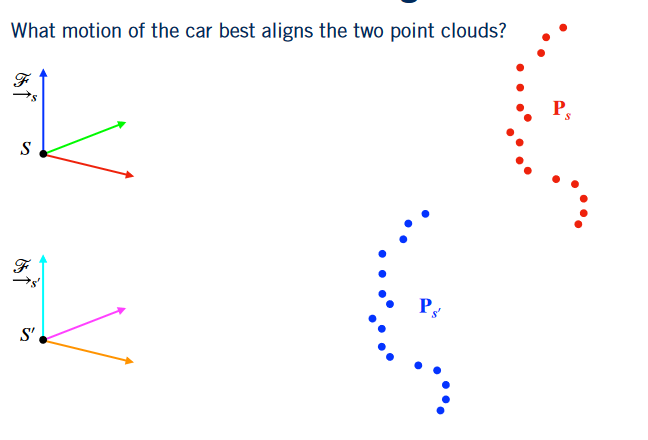
\includegraphics[width=8cm]{img/icp.png}
    \caption{Illustration of point registration for state estimation task}
    \label{fig:state_estimate}
\end{figure}

Now, we have some problems - we don't always know which points correspond to another from our two sets of points. So, if we assume that our transformation was very tiny, we can reduce the possibilities of what point corresponds to another. We can then set an initial GUESS for the transformation - an identity transform and then work with this to find the ideal transform. The intuition is when the optimal motion is found, corresponding points will be closer to each other than to other points. For small displacements, this heuristic works: For each point, the best candidate for a corresponding point is the point that is closest to it right now.

\textbf{Procedure:}

\begin{itemize}
    \item Get an initial guess for the transform $\{\hat{R}_s^s', t\}$
    \item Associate each point with a corresponding one.
    \item Solve for optimal transformation
    \item Repeat till convergence
\end{itemize}

The key thing here is the knowledge of corresponding points is important. Sometimes it is known, sometimes not. In the former case, we have to directly aim for a solution, but in the latter we work on first estimating some correspondences and then looking for a transform (like the algo above). This guesstimate can be found by drawing a normal from a point and seeing what corresponding point we hit. This iterative algorithm is ICP. Look at \href{https://www.notion.so/Point-Cloud-Registration-Iterative-Closest-Point-a25686ce1a11409d838d47bcac43ab4b}{Shubodh's notes from Mobile Robotics} for more explanation about ICP.

As mentioned earlier, there are two things:

\textbf{Known correspondences}

Here, we have the luxury of posing this as an equation that must be solved. If we assume that our points are $\{p_i\}$ and $\{q_j\}$, then we can find the centroid (or mean of points) of each of these sets. We can safely state that the transformation between these points is the same that the centroid will undergo.

We then do a singular value decomposition. The solution for the problem then becomes $UV^T$. Page 10 of \href{https://arxiv.org/pdf/1705.09785.pdf}{this paper by MK} has a real clear explanation on why that is. As mentioned earlier, the translation between centroids is equivalent to the translation between ALIGNED frames. This information lets us solve for just the rotation matrix.

\textbf{Unknown correspondences}

If the correct correspondences are not known, it is generally impossible to determine the optimal relative rotation and translation in one step. The algorithm converges if starting positions are “close enough”. There are various matching algorithms, some of which are shown \href{https://www.notion.so/Point-Cloud-Registration-Iterative-Closest-Point-a25686ce1a11409d838d47bcac43ab4b#acdbf05aa6834446bc0812b2ae3f0f40}{here} - Closest-point, normal shooting, etc. This data association has a very high impact on convergence and speed.

It is possible to use feature extractors and have feature correspondences as well. But this is easier said than done since we will be dealing with LiDAR data often for point clouds.

Some variants of ICP can be seen in Shubodh's notes. 

\subsection{Solving ICP}

We tend to consider overdetermined systems here, we have $m\geq n$. We are solving for something like $Ax=b$ where $A$ is a full rank matrix (rank = $\min (m, n)$. There are a lot of ways to solve for this regularly but for the purpose of discussion, we will try to find the optimal $A$. This matrix just needs to get most of the transformations right, so we pose it as a least squares chapter as seen in the last chapter (and can solve in that way as well).

In ICP, we are solving for 6 variables. Each point gives rise to 3 equations, so with two points we can technically solve for it. But our point cloud is more dense than that, so we end up with an overdetermined solution. 

A SVD solution to ICP has already been shown in that earlier paper by MK.

\subsubsection{ICP as Least Squares}

Let's assume that we have a set of m points in frame I, J - $\{P_i\}$, $\{Q_j\}$.

\begin{equation}
    \Vec{P_i} = R\Vec{Q_i} + t
\end{equation}

We can represent the R matrix using Z-Y-X euler angles for ease. But this has non-linear terms - many $\cos$ and $\sin$. So, for ease, we make a small angle assumption (like before) because of which, we can say that:

\textit{He mentions that we could have linearised instead by taking the Jacobian. And, using Taylor approximation leads to small angle assumption.}

$\cos \alpha = 1$, $\sin \alpha = \alpha$ and so on. So, the resulting rotation matrix becomes:

\begin{equation}
\begin{bmatrix}
1 & -\alpha & \beta \\
\alpha & 1 & -\gamma \\
-\beta & -\gamma & 1\\
\end{bmatrix}
\end{equation}

Hence, we can rewrite our transformation between frames as :

\begin{equation}
\begin{bmatrix}
1 & -\alpha & \beta \\
\alpha & 1 & -\gamma \\
-\beta & -\gamma & 1\\
\end{bmatrix} \begin{bmatrix}Q_{x_1} \\ Q_{y_1} \\ Q_{z_1}\end{bmatrix} + \begin{bmatrix}t_x \\ t_y \\ t_z\end{bmatrix} = \begin{bmatrix} P_{x_1} \\ P_{y_1} \\ P_{z_1} \end{bmatrix}
\end{equation}

\textit{t is the translation of Q wrt P}

Now, we can easily write this in the form of $Ax=b$. This ends up becoming:

\begin{equation}
    \begin{bmatrix}
    -Q_{y_1} & Q_{z_1} & 0 & 1 & 0 & 0 \\
    Q_{x_1} & 0 & -Q_{z_1} & 0 & 1 & 0 \\
    0 & - Q_{x_1} & Q_{y_1} & 0 & 0 & 1 \\
    \end{bmatrix} \begin{bmatrix}
    \alpha \\
    \beta \\
    \gamma \\
    t_x \\
    t_y \\
    t_z \\
    \end{bmatrix} = \begin{bmatrix}
    P_{x_1} - Q_{x_1} \\
    P_{y_1} - Q_{y_1} \\
    P_{z_1} - Q_{z_1} \\
    \end{bmatrix}
\end{equation}

This is just for one correspondence, so we can stack each correpsondence such that we get:

\begin{equation}
    \begin{bmatrix}
    A^1 \\
    A^2 \\
    \vdots \\
    A^m
    \end{bmatrix} X = \begin{bmatrix}
    b^1 \\
    b^2 \\
    \vdots \\
    b^m
    \end{bmatrix}
\end{equation}

\textit{Why are we doing n points again? Because some correspondences may be wrong, so we want more data points.}

Check the last chapter to see how SVD can be used to solve least squares problems. There are various ways to go about solving ICP.

BUT, there is a problem here - we had to make a small angle assumption. Let's express this problem in a new way now:

\begin{equation*}
    Ax = b
\end{equation*}

\begin{equation}
    \begin{bmatrix}Q_{x_1} & Q_{y_1} & Q_{z_1} & 000 & 0 & 0 & 0 & 1 & 0 & 0 \\
    \hdots \\
    \hdots \\
    \end{bmatrix} \begin{bmatrix}r \\ \vdots \\ t\end{bmatrix} = \begin{bmatrix}P_{x_1} \\ P_{y_1} \\ P_{z_1}\end{bmatrix}
\end{equation}

The above equation essentially stretches the rotation matrix, and stacks it on top of the translation vector. We are able to write $P = RQ + t$ in this form as a result. 

Now, why can't we use this to solve as a least squares problem. We just have more variables - 12 here (the rotation, translation vector). The variables aren't independent! There are many constraints that come with the values being a part of rotation matrix. These constraints are $RR^T=I$, $\norm{R_i}=1$. These constraints make the solution a non-convex one (ref prev chapter for explanation). This is a manifold optimization problem, consider a locally euclidian space, take it to a tangential space and work there and return to eulician space. Note that rotation matrices aren't euclidian (you cant add rotations to combine rotations for instance). 

In principle, we can linearize the equation above, and use the Jacobian to write it using Taylor series. 

\textit{We always made a full rank assumption here (which holds true because of noise as discussed in some other chapter), but this can fail if the points are coplanar or colinear (depends on the situation).}

\subsection{Multiview ICP}

How to get the right poses AND the map from noisy estimates of poses and the map? 

$T_0 = \begin{bmatrix}I & 0 \\ 0 & 1\end{bmatrix}$ is the origin. We are generally using homogenous equations. Here, the rotation is identity, indicating that we are at origin (translation is origin too). 

The robot has move, its estimating position, and estimating point clouds but it makes errors!

We will pose ICP as a multiview optimization to alleviate the error.

The insight: If there is a grame $\{q\}$ in which the depth measurements and the point cloud $\hat{X_{qj}}, j=\{1,\hdots,n\}$ are particularly noiseless. Can this be used to alleviate other views in terms of poses and 3D pooints estimated in those views. 

If a set of n points are viewed in m frames or observations what is the best estimate for these n points and m poses. - Multiview aggregation and Multiview consistency.

\section{Loop Closures}

\href{https://www.notion.so/Loop-Closure-8ab30a4560ea4d859c92c515c99ef70a}{Summer school loop closure notes} can be found here - Udit made them.

\begin{figure}[h]
    \centering
    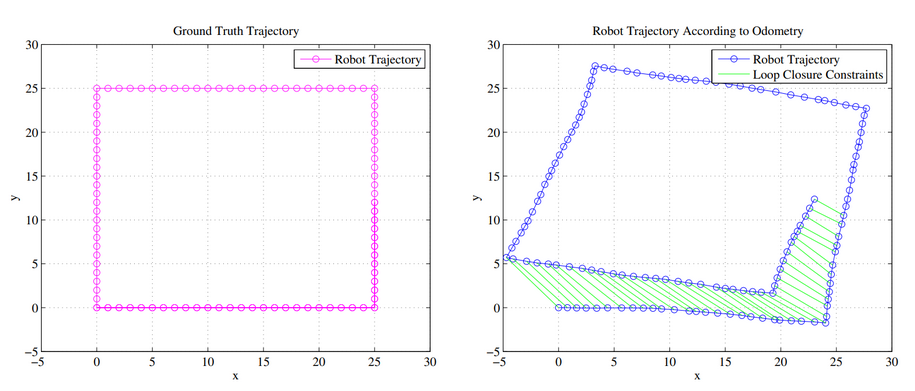
\includegraphics[width=12cm ]{img/loop_closure.png}
    \caption{Loop Closure}
    \label{fig:loop_closure}
\end{figure}

Information that is fed into SLAM is relative to the position of the robot. So, as we move along, the predictions we make are dependent on the previous positions. As a result, errors can accumulate over time causing problems. In contrast to this, the shape of the room is fixed and won't change. 

Now, assume that the robot moves along a closed loop, returns to the start of the loop but it may not know this yet.  Look at the image above, it shows the actual trajectory of the robot. But, using odometry measurements, it predicts the positions on the right. Loop closure works to enforce constraints on the mapping between points that are revisited. This is a challenging problem because it has to detect same locations (data-association again gargh).

If we consider SLAM as a conditionaly dependency graph - visualize this as a set of nodes over time, now after moving, some nodes will be repeated. Loop closure helps ensure that the two repeated nodes similar.

A  robot  performing  odometry  and  neglecting  loop closures interprets the world as an “infinite corridor”. Look at page 2 of \href{https://arxiv.org/pdf/1606.05830.pdf#page=3&zoom=110,106,607}{this review paper} to see why Loop closure is important in more detail.

On the note of data association, one technique that is used is Bag of Visual Words

\subsection{Bag of Visual Words}

Imagine that you have some important tasks such as finding images with a theme or text with some tags. This is a hard task where linearly searching for similarity isn't feasible. The solution is to extract some good features and construct a set of them, and construct a histogram based on the occcurences of these features. Now, using this lower dimension representation of our data, we can perform our operations sooner.

So, we extract feature descriptors from SIFT/ORB, cluster using K-Means to get final visual words in a dictionary. The centroids form the required dictionary.

We can use these histograms to compare our locations. This is often done using cosine similarity (another measure of distance) = $\frac{x^Ty}{\norm{x}\norm{y}}$.

As always, we want words that have high variance - if everything has something in common, why does it help us? 

\section{Review of Visual Odometry}

Motion estimation is called visual odometry - estimating our poses given corresponding images. This can be done using 2D-2D, 3D-3D and even 2D-3D methods.

Considering the overwhelming number of algorithms mentioned so far, a quick review:

\begin{itemize}
    \item 2D-2D: Epipolar Geometry via Fundamental Matrix
    \item 3D-2D: Compute the 3d point given position of points in images and camera matrices
    \item 3D-2D: Given 3D points in world frame and 2D correspondences in camera frame, estimate camera motion/pose.
    \item 3D-3D: ICP
\end{itemize}

\section{Frontend}

\begin{figure}[h]
    \centering
    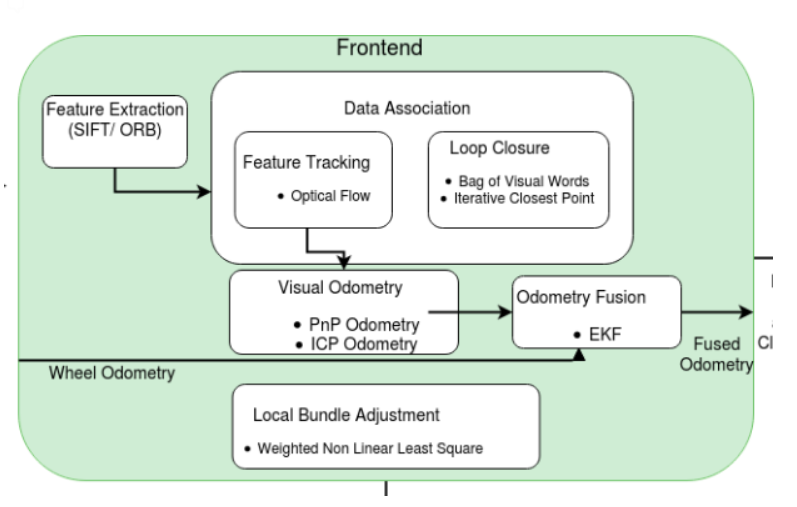
\includegraphics[width=12cm]{img/frontend.png}
    \caption{Frontend}
    \label{fig:frontend}
\end{figure}

The SLAM frontend detects features, matches them, and estimates motion using one of the algorithms mentioned above. Feature extraction can happen using something like SIFT. In the context of SLAM, good features are those that remain stable after camera motion. Harris corner is bad here cause it won't work well. We need points that are repeatable, distinct in representation, or local. ORB happens to be very fast. There are some direct methods for SLAM as well, seen \href{https://www.notion.so/SLAM-Frontend-Visual-Odometry-bd7dbccb797f442f955f450044ee200f#5346a971d36a4ac386c772228c7fe3bd}{here in Shubodh's notes.}

We can use Kalman filters to fuse multiple sensor streams.

\section{Backend}

\begin{figure}[h]
    \centering
    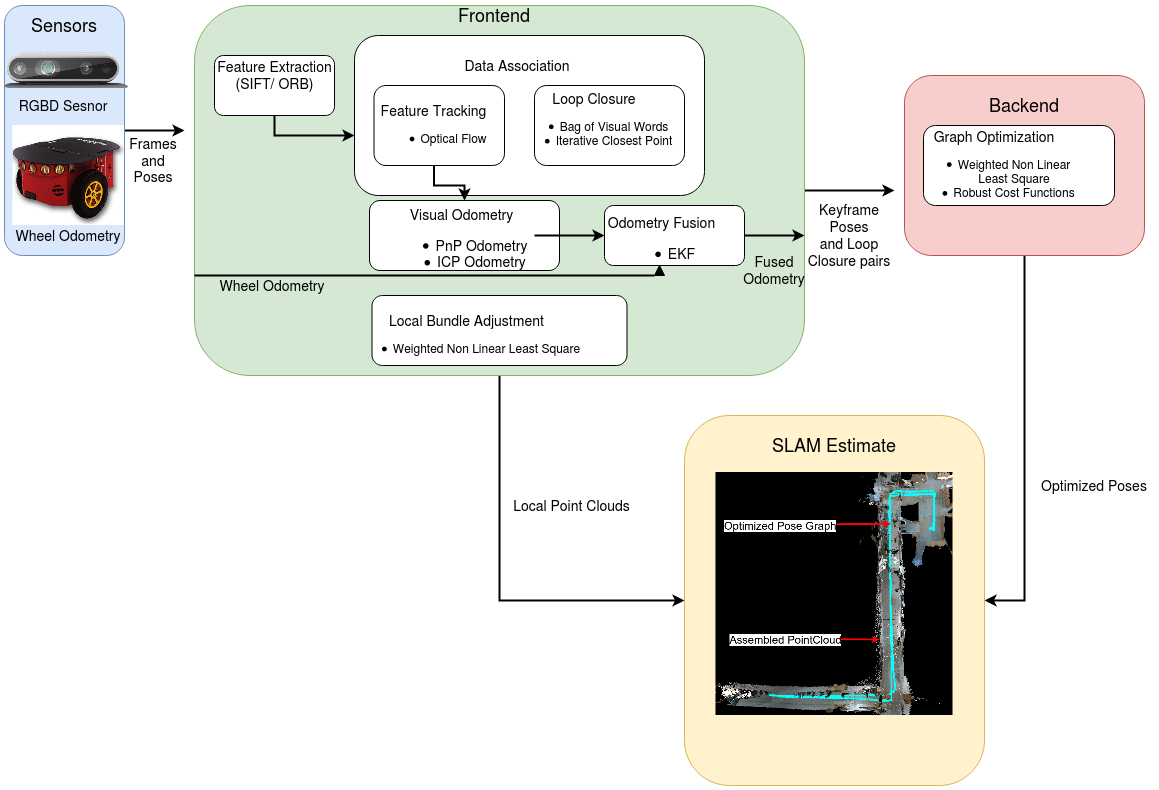
\includegraphics[width=12cm]{img/backend.png}
    \caption{Full Picture}
    \label{fig:slam}
\end{figure}

Now that we've seen the broad picture, we can see how various components will interact with each other. The SLAM Backend provides an interface to graph construction and optimization tools. It essentially forms the map of our SLAM system and uses pose estimates from the visual odometry to form the nodes of a graph. It also corrects drift in the VO estimates when the Place Recognition node flags a match between views. There's a lot math here and various approaches - using Bundle Adjustment or Pose Graph estimation.

\section{State of the Art and Applications}

SLAM has a wide range of applications in the mapping domain - \href{http://www.informatik.uni-bremen.de/agebv2/downloads/published/freseki10.pdf}{as shown well in this paper}. In augmented reality, where graphics are put on top of a camera image, we need to know the cameras position in the world. \href{https://sci-hub.tw/10.1109/ISMAR.2007.4538852}{The introduction to this paper on AR} has some insights into the application of SLAM for AR.

\subsection*{MonoSLAM}

MonoSLAM was the first ever monocular SLAM system. The frontend was very sparse feature point tracking. The backend was primarily done using Kalman filter. Given previous state of the camera and current landmarks, it would give the current state of the camera. 

\subsection*{ORD-SLAM}

This uses ORB feature extractor to get features. The entire system is calculated around ORB features including visual odometry and ORB dictionaries for loop detection.

\subsection*{Semi-Direct Visual Odometry}

This is a combination of keypoints (not descriptors) and information around the keypoints using direct methods. Direct methods tend to use the entire image. Just as the name suggests, it is not a complete SLAM pipeline. If there are some errors in odometry, the errors will propogate since there is no backend optimization here or loop closures here.

\subsection*{RTAB-Map}

RTABMAP is a classic solution in the RGB-D SLAM. It implements feature-based visual odometry, bag-of-words-based loop detection, back-end pose map optimization, and point cloud and triangular mesh maps. 

Support for multi-session mapping is provided, which allows the SLAM approach to initialize a new map with its own referential on startup, and when a previously visited location is encountered, a transformation between the two maps can be computed. This can be seen as a fancier version of loop closure as using ICP or so, we can combine maps that were separately made.

\subsection*{Semantic SLAM \& Future}

Till now, we've only explored SLAM that localizes and maps. Semantic SLAM will also classify items in the map giving the SLAM three layers - localization, mapping, and classification.

In 3D dynamic scene graphs, there are multiple layers to the SLAM - metric semantic mesh, objects and agents, places and structures, rooms, and buildings.

As per Andrew Davidson, there is robust localization, dense mapping and semantic understanding of the world. 

It can be said that semantic helps SLAM and SLAM helps semantics. Why?

So far, we've looked at static SLAM but when the environment is dynamic - the algorithms are bound to fail. With semantics, we may segment out humans and other dynamic objects. These semantics are critical to understanding the environment obviously - just as we are aware of moving objects in life. 

Now, typically in deep learning we have a series of images that aren't explicitly related. But with SLAM information, we can warp images to obtain new images (similar to ones that are seen) and we needn't make another forward pass.